\let\negmedspace\undefined
\let\negthickspace\undefined
\documentclass[journal]{IEEEtran}
\usepackage[a5paper, margin=10mm, onecolumn]{geometry}
\usepackage{tfrupee} % Include tfrupee package

\setlength{\headheight}{1cm} 
\setlength{\headsep}{0mm}     

\usepackage{gvv-book}
\usepackage{gvv}
\usepackage{cite}
\usepackage{amsmath,amssymb,amsfonts,amsthm}
\usepackage{algorithmic}
\usepackage{graphicx}
\usepackage{textcomp}
\usepackage{xcolor}
\usepackage{txfonts}
\usepackage{listings}
\usepackage{enumitem}
\usepackage{mathtools}
\usepackage{gensymb}
\usepackage{comment}
\usepackage[breaklinks=true]{hyperref}
\usepackage{tkz-euclide} 
\usepackage{listings}
\def\inputGnumericTable{}                                 
\usepackage[latin1]{inputenc}                                
\usepackage{color}                                            
\usepackage{array}                                            
\usepackage{longtable}                                       
\usepackage{calc}                                             
\usepackage{multirow}                                         
\usepackage{hhline}                                           
\usepackage{ifthen}                                           
\usepackage{lscape}
\usepackage{circuitikz}
\tikzstyle{block} = [rectangle, draw, fill=blue!20, 
    text width=4em, text centered, rounded corners, minimum height=3em]
\tikzstyle{sum} = [draw, fill=blue!10, circle, minimum size=1cm, node distance=1.5cm]
\tikzstyle{input} = [coordinate]
\tikzstyle{output} = [coordinate]


\begin{document}

\bibliographystyle{IEEEtran}
\vspace{3cm}

\title{7.4.3}
\author{AI25BTECH11036-SNEHAMRUDULA}
 \maketitle
{\let\newpage\relax\maketitle}
\renewcommand{\thefigure}{\theenumi}
\renewcommand{\thetable}{\theenumi}
\setlength{\intextsep}{10pt} 
\numberwithin{equation}{enumi}
\numberwithin{figure}{enumi}
\renewcommand{\thetable}{\theenumi}
\textbf{Question}:\\
\textbf{Q.}\;
From the origin chords are drawn to the circle 
\begin{align}
    \brak{u-\myvec{1\\0}}^\top \brak{u-\myvec{1\\0}} = 1
\end{align}
The equation of the locus of the mid-points of these chords is to be found.


\solution\\

1.The given circle equation is
\begin{align}
    \vec{u}^\top \vec{u} -2\myvec{1&0}\vec{u} = 0
\end{align}
which can be expressed in standard form as
\begin{align}
    \vec{u}^\top \vec{u} + 2\vec{c}^\top\vec{u} + f = 0
\end{align}
where
\begin{align}
    \vec{c} = \myvec{-1\\0}, \quad f = 0
\end{align}
2.A chord of this circle passing through the origin $O=\myvec{0\\0}$ has midpoint $\vec{m}$.  
From the property of chord bisectors:
\begin{align}
    \vec{m}^\top \vec{c} + \vec{m}^\top \vec{m} = 0
\end{align}
3.Substituting $\vec{c}=\myvec{-1\\0}$,
\begin{align}
    -m_1 + m_1^2+m_2^2 = 0
\end{align}
4.Hence, the locus of $\vec{m}$ is
\begin{align}
    \vec{m}^\top \vec{m} = m_1
\end{align}
Thus, the locus of the midpoints is the circle 
\[
m_1^2 + m_2^2 = m_1,
\]
i.e., a circle with center $\left(\tfrac{1}{2},0\right)$ and radius $\tfrac{1}{2}$.

\end{solution}
\begin{figure}[h!]
    \centering
    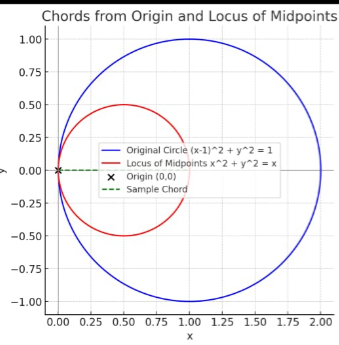
\includegraphics[height=0.5\textheight, keepaspectratio]{fiig7.4.3.png}
    \label{figure_1}
\end{figure}
 
\end{document}